\section{Web App}

The web application was developed using \textbf{Flask}, a lightweight Python web framework, and communicates with the Oracle database using the \texttt{oracledb} library. The application provides a user-friendly dashboard with multiple forms for data entry and query operations. Each form submission triggers corresponding PL/SQL procedures stored in the database to perform the required operations. Database credentials are securely loaded from environment variables, and Jinja2 templating is used to render dynamic HTML pages. The user interface was enhanced using \textbf{Bootstrap 5}, providing a responsive, modern design with organized card-based layouts, styled form controls, and dismissible alert messages for user feedback.

\begin{figure}[H]
    \centering
    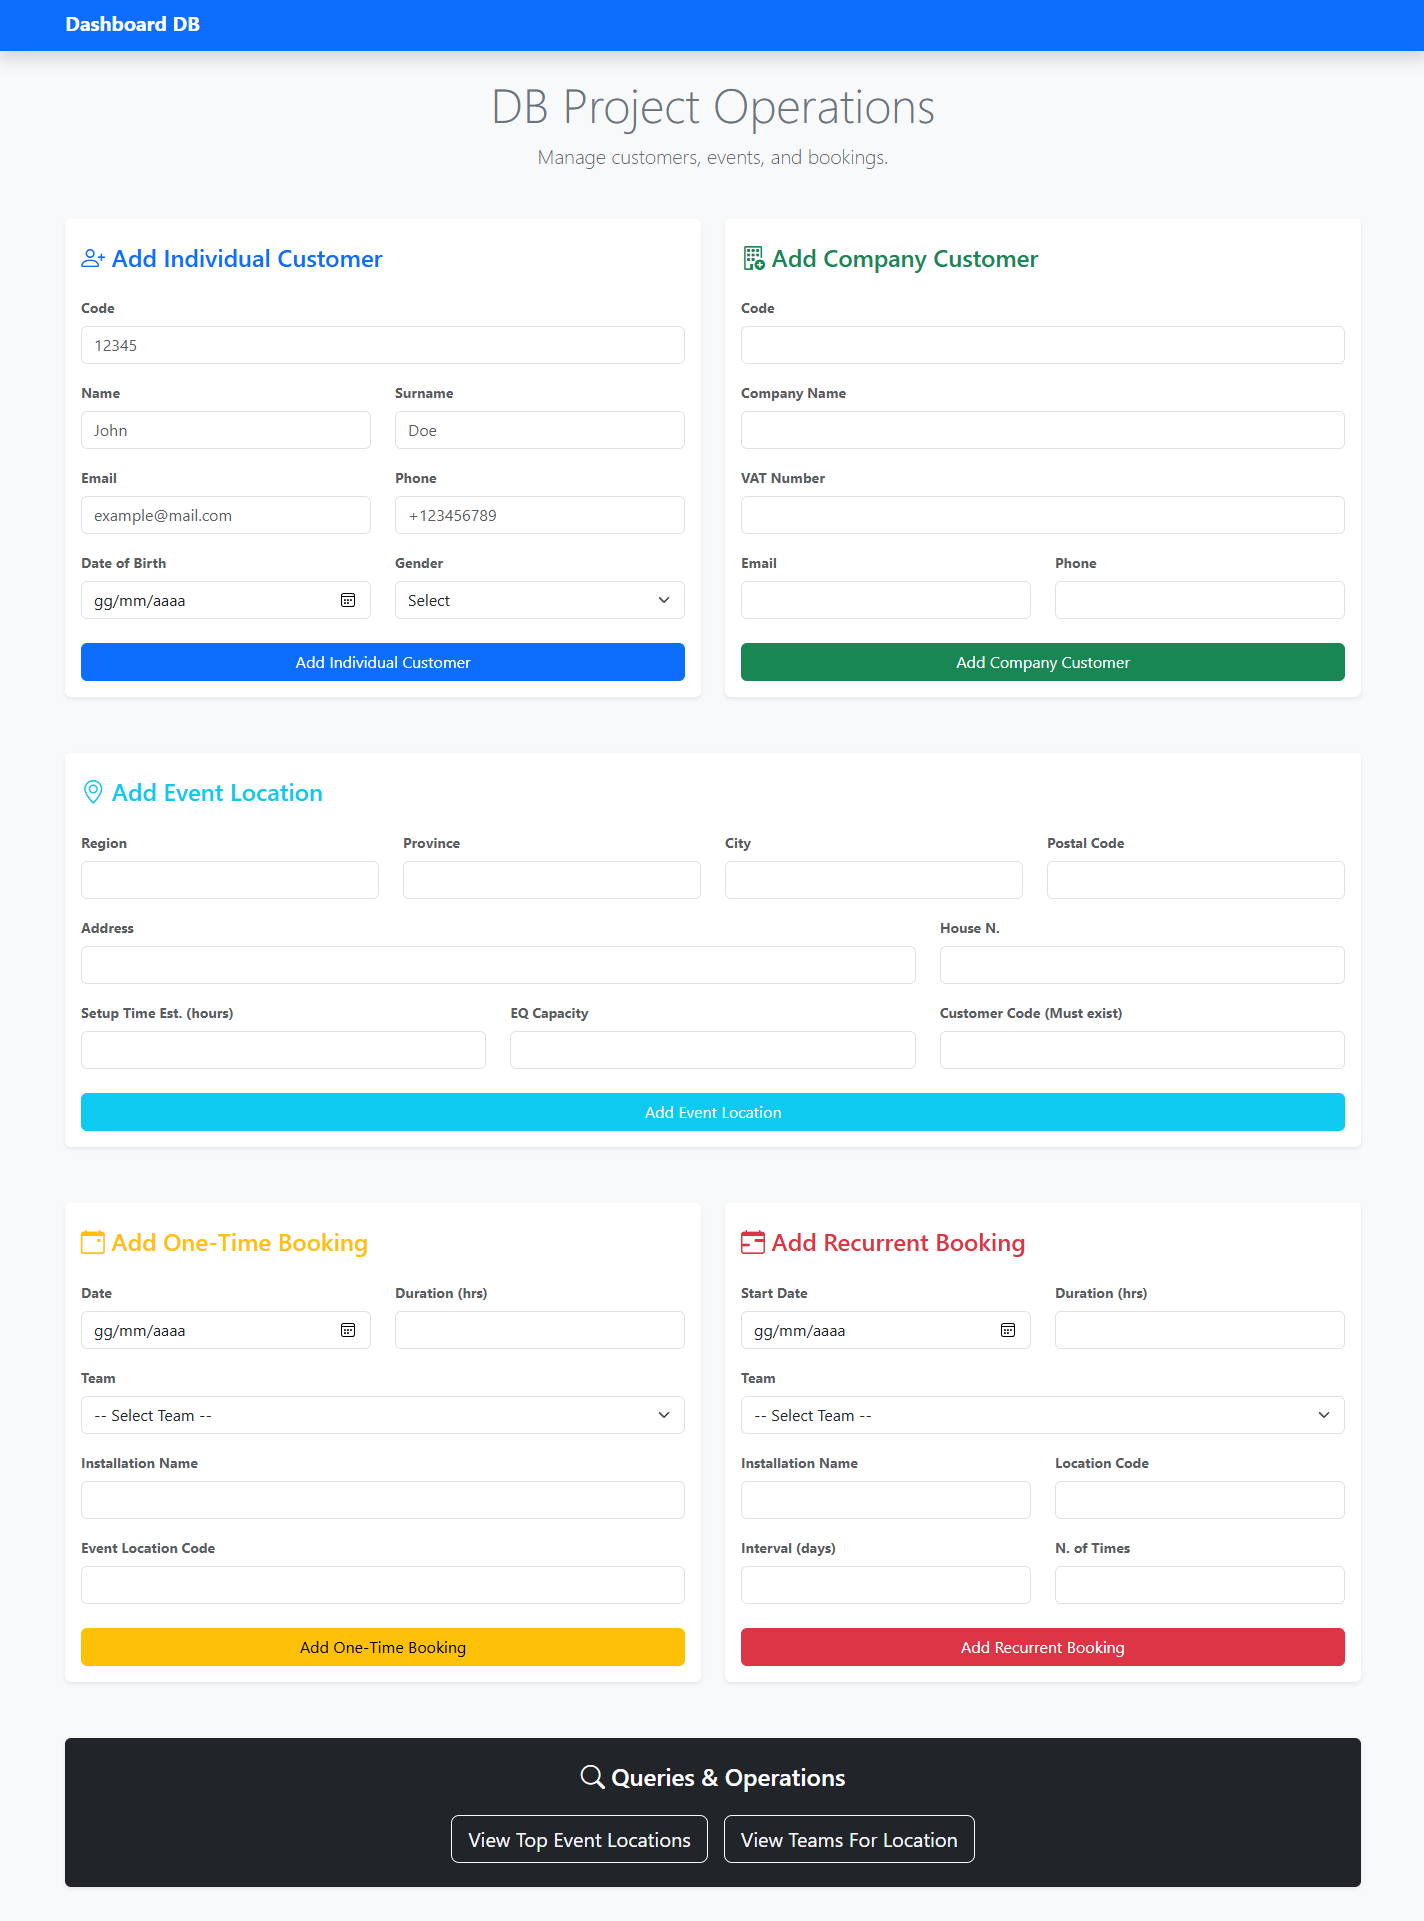
\includegraphics[width=0.95\textwidth]{./rsc/webapp-home.png}
    \caption{Screenshot of the home page of the web application}
    \label{fig:webapp-home}
\end{figure}

\begin{figure}[H]
    \centering
    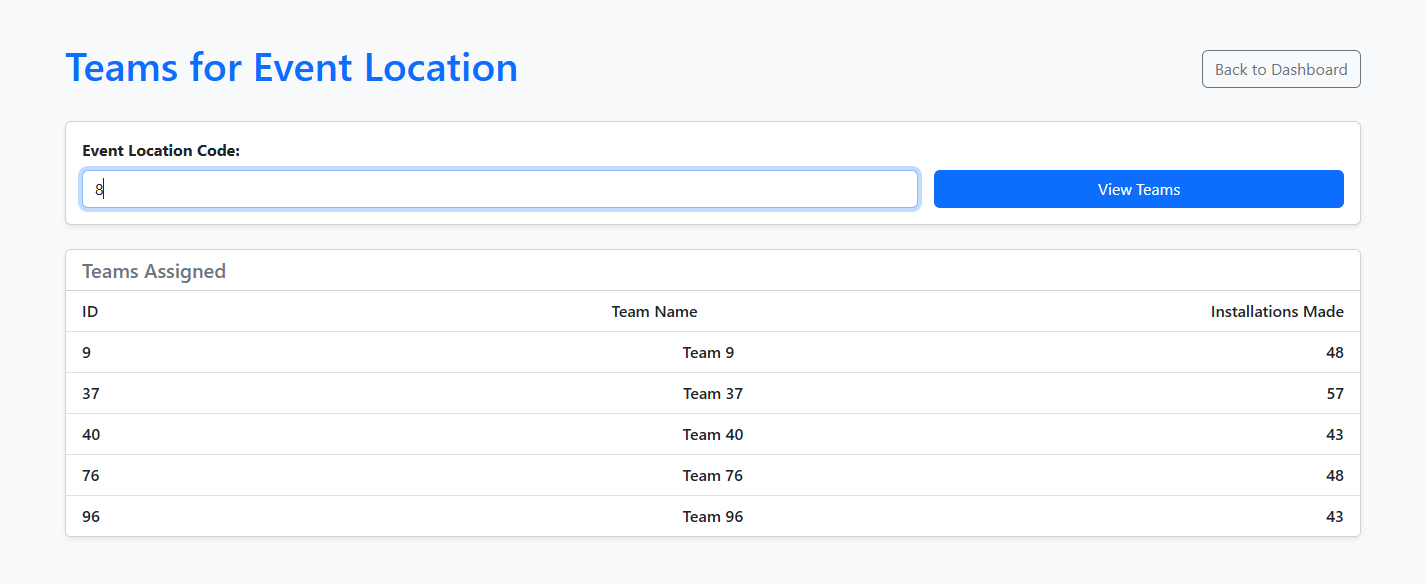
\includegraphics[width=0.95\textwidth]{./rsc/webapp-teams.png}
    \caption{Screenshot of the execution of operation \ref{op4}}
    \label{fig:screenshot-op4}
\end{figure}

\begin{figure}[H]
    \centering
    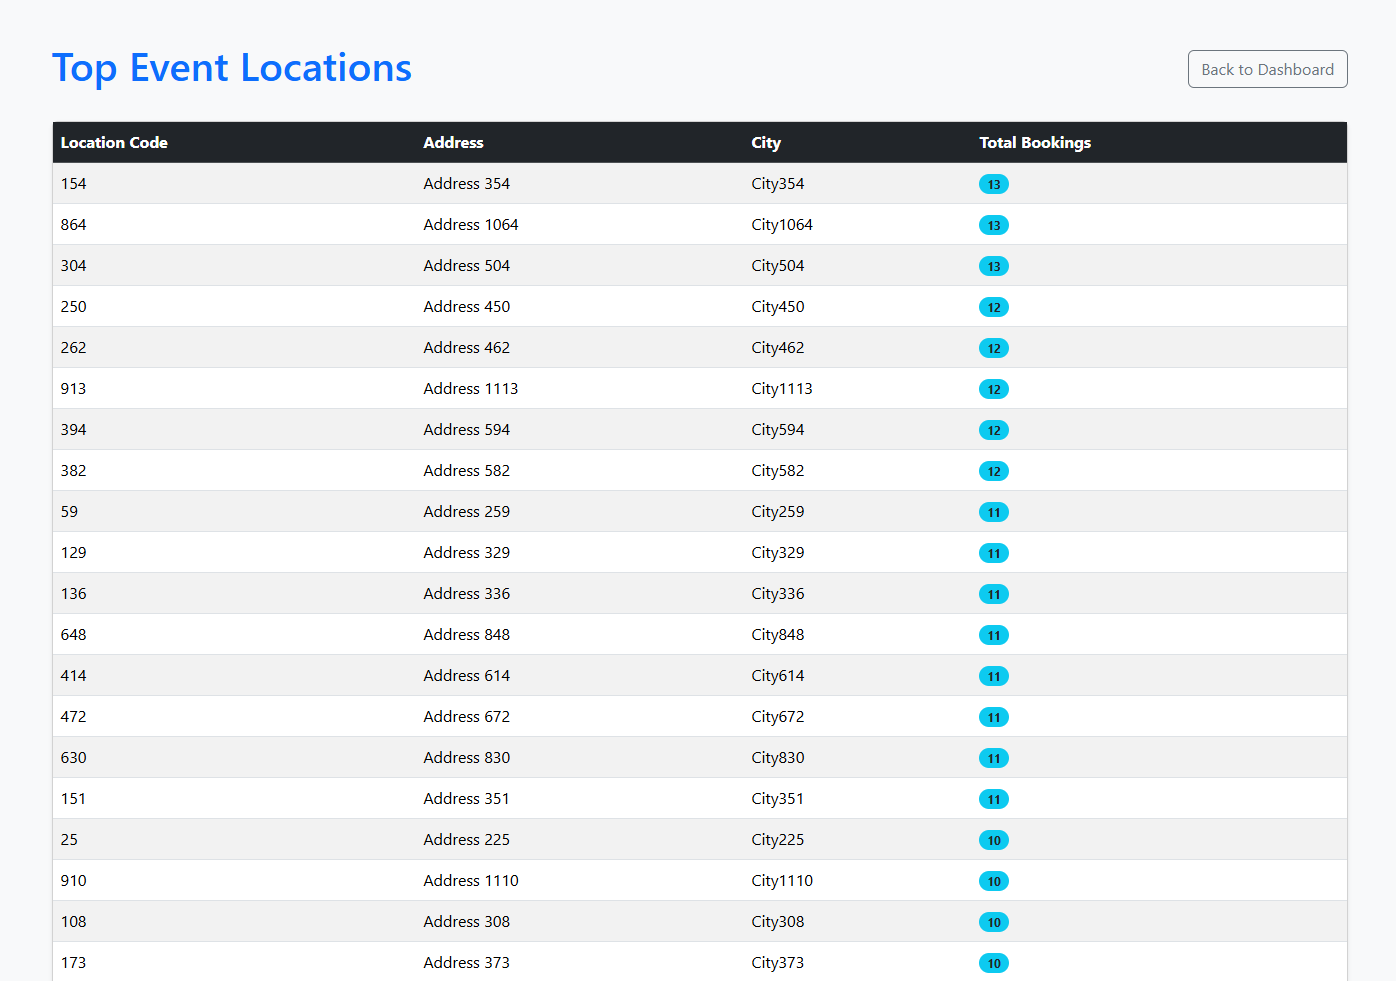
\includegraphics[width=0.95\textwidth]{./rsc/webapp-top-locations.png}
    \caption{Screenshot of the execution of operation \ref{op5}}
    \label{fig:screenshot-op5}
\end{figure}

